\documentclass[12pt,a4paper]{article}
\usepackage{amsmath,amsthm,amsfonts,amssymb,amscd}
\usepackage{times}              
% Use Times New Roman
\usepackage{graphicx}           
% Enhanced support for images
\usepackage{float}              
% Improved interface for floating objects
\usepackage{booktabs}           
% Publication quality tables
\usepackage{xcolor}             
% Driver-independent color extensions
\usepackage{geometry}           
% Customize document dimensions
\usepackage{fullpage}           
% all 4 margins to be either 1 inch or 1.5 cm
\usepackage{comment}            
% Commenting
\usepackage{minted}             
% Highlighted source code. Syntax highlighting
\usepackage{listings}           
% Typeset programs (programming code) within LaTeX
\usepackage{lastpage}           
% Reference last page for Page N of M type footers.
\usepackage{fancyhdr}           
% Control of page headers and footers
\usepackage{hyperref}           
% Cross-referencing 
\usepackage[small,bf]{caption}  
% Captions
\usepackage{multicol}
\usepackage{tikz}               
% Creating graphic elements
\usepackage{circuitikz}         
% Creating circuits
\usepackage{verbatim}          
% Print exactly what you type in
\usepackage{cite}               
% Citation
\usepackage[us]{datetime} 
% Various time format
\usepackage{blindtext}
% Generate blind text
\usepackage[utf8]{inputenc}
\usepackage{array}
\usepackage{makecell}
\usepackage{tabularx}
\usepackage{titlesec}
\usepackage{enumitem}
\usepackage[brazil]{babel}

\input{defs.tex}



\begin{document}

\textcolor{UM_Brown}{
\begin{minipage}{0.1\textwidth}
    \begin{flushleft}
        \includegraphics[height=3.5cm]{Figures/UFRN_Brasao.png}
    \end{flushleft}
\end{minipage}
\begin{minipage}{0.8\textwidth}
    \begin{center}
        \textbf{\Large Laboratório de Física Moderna}\\
        \vspace{5pt}
        Relatórios 1 - 5 \\
        \vspace{20pt}
        \textit{Gabriel Wendell Celestino Rocha} \\
        \vspace{5pt}
        \textit{Vinícius Câmara Filgueira}
    \end{center}
\end{minipage}
\vspace{10pt}
\hrule
}



%%%%%%%%%%%%%%%%%%%%%%%%%%%% 
\section*{Atividade 1 - Tubo de Crookes}
\begin{enumerate}

    \item Considere a equação de Goldstein-Wehner que relaciona a pressão $P$ no interior do tubo de Crookes com a largura $d_k$ da $k$-ésima estria formada:
    \begin{equation} \label{eq:Crookes_pressure}
        \frac{d_{k}}{R}=\frac{C}{\left(P\cdot R\right)^{n}}\implies P\cdot R=\left(\frac{R\cdot C}{d_{k}}\right)^{1/n}\quad\therefore\quad\boxed{P=R^{\frac{n+1}{n}}\cdot\left(\frac{C}{d_{k}}\right)^{1/n}}\text{ }
    \end{equation}
    onde $R=1.4$ cm é o raio inteiro do tubo de Crookes, $C=1.2\text{ }(\text{Torr}\cdot\text{cm})^n$ é uma constante que depende do gás usado no experimento, $n=0.32$ é um coeficiente que também depende do gás usado no experimento.
    
    Estamos interessados em calcular a pressão no interior do tubo devido à primeira estria, logo, estamos interessados em obter o valor de $d_1$. Diante disso, com base na Figura \ref{fig:ativ1}, podemos estimar a largura da primeira estria como sendo $d_1=705\text{ mm}-695\text{ mm}=10\text{ mm}=1.0\text{ cm}$.
    
    \begin{figure}[htp!]
        \centering
        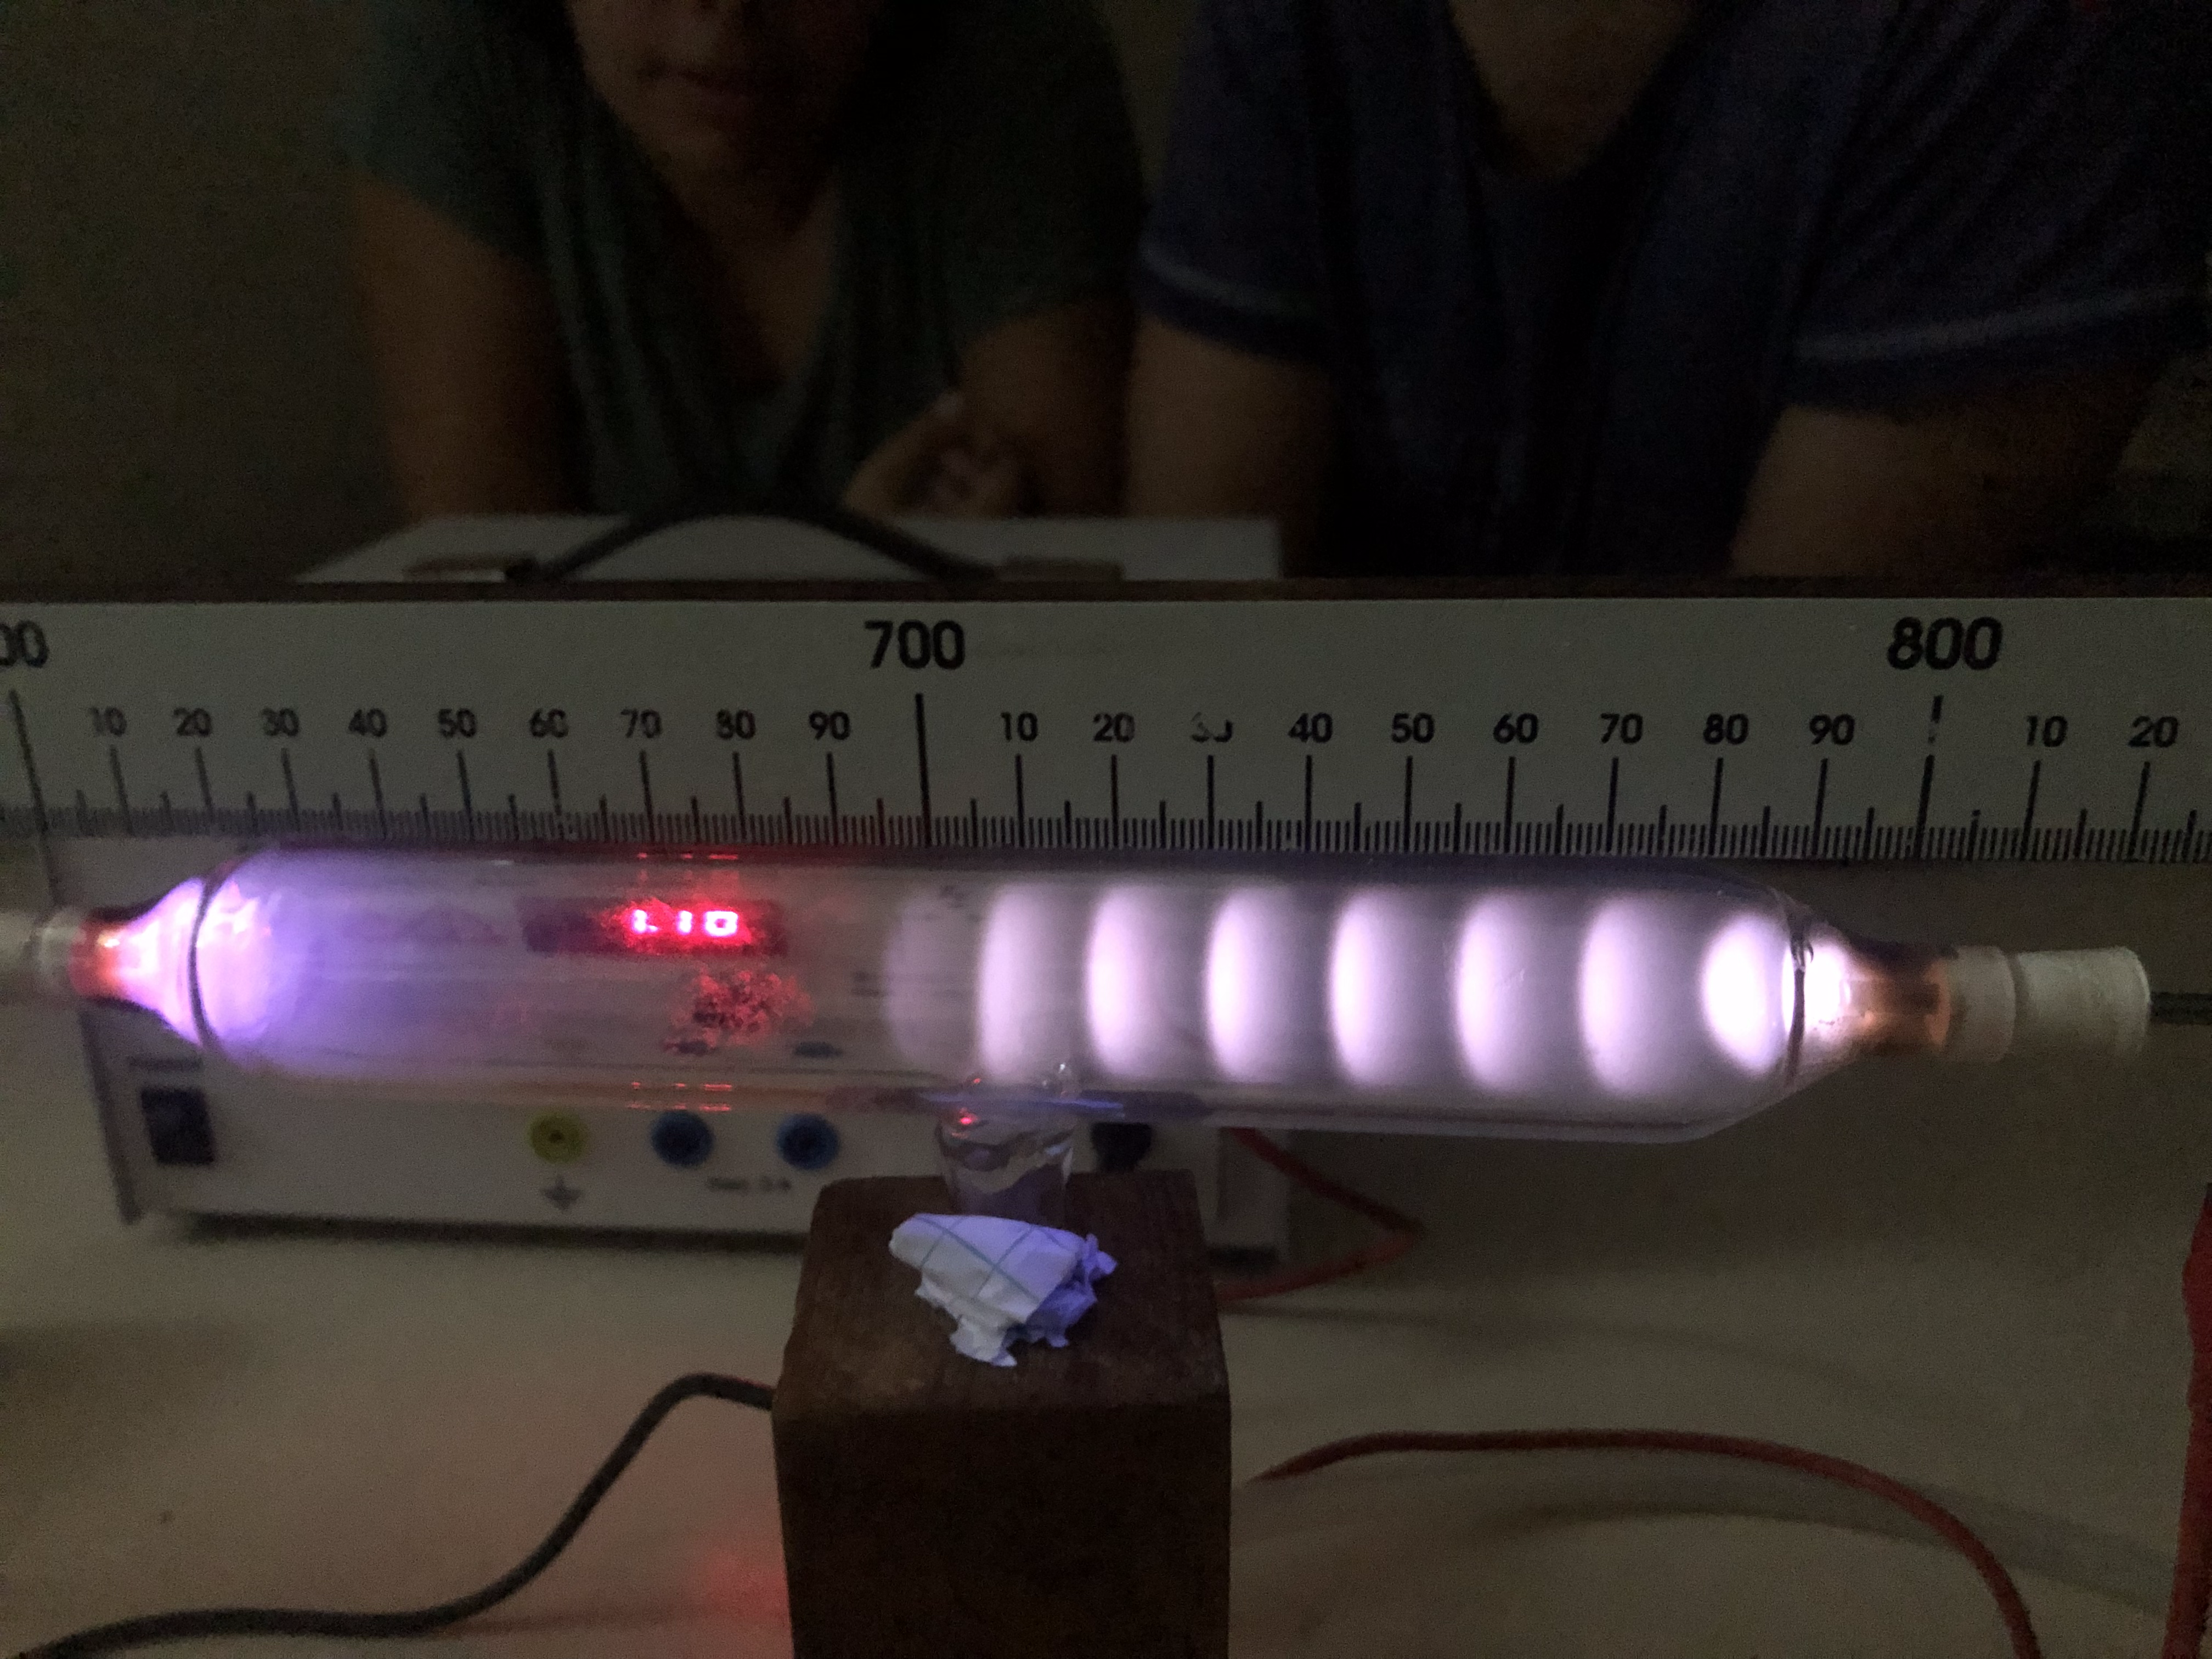
\includegraphics[width=0.7\linewidth]{Figures/Fig1.png}
        \caption{Experimento do tubo de Crookes.}
        \label{fig:ativ1}
    \end{figure}
    
    Convertendo todas as unidades para que fiquem de acordo com as unidades padrão do Sistema Internacional de Unidades (SI) e substituindo na Equação (\ref{eq:Crookes_pressure}), obtemos
    \begin{equation} \label{eq:pressure}
        P=\left(1.4\text{ cm}\right)^{\frac{1.32}{0.32}}\cdot\left(\frac{1.2\text{ Torr}^{0.32}\cdot\text{cm}^{-0.32}}{1.0\text{ cm}}\right)^{1/0.32}\quad\therefore\quad\boxed{P\approxeq5.634\text{ Torr}}
    \end{equation}
    \begin{flushright}
        $\blacksquare$
    \end{flushright}



    \item Sendo $760$ Torr a pressão atmosférica (externa ao tubo), nota-se que a pressão no interior do tubo é muito menor que a pressão atmosférica como já era de se esperar uma vez que o ar no interior do tubo deve ser o mais rarefeito possível. Para determinarmos a magnitude no qual a pressão no interior do tubo é menor basta calcularmos a razão:  
    \begin{equation} \label{eq: Pressure_ratio}
        \frac{P_{atm}}{P}=\frac{760\text{ Torr}}{5.634\text{ Torr}}\approxeq 134.88.
    \end{equation}
    \begin{flushright}
        $\blacksquare$
    \end{flushright}

    Ou seja, a pressão no interior do tubo de Crookes é cerca de 135 vezes menor que a pressão atmosférica.



    \item Comecemos determinando uma expressão analítica para a velocidade $v$ de um elétron de carga $q$ e massa $m$ quando submetido a uma diferença de potencial $\Delta V$.

    Pelo teorema do trabalho-energia podemos escrever (note que estamos assumindo que o elétron parte do respouso):
    \begin{equation} \label{eq:e_vel}
        F\cdot d=\Delta K\implies Eq\cdot d=\frac{1}{2}m_ev_e^{2}\quad\therefore\quad\boxed{v_e=\sqrt{\frac{2q\Delta V}{m_e}}}
    \end{equation}
    \begin{flushright}
        $\blacksquare$
    \end{flushright}

    Sabe-se que o elétron possui massa de repouso de $m_e=9\cdot10^{-31}$ kg e carga (em módulo) igual a $q=1.6\cdot10^{-19}$ kg. Sendo $\Delta V=2500$ Volts, temos que a velocidade atingida pelo elétron é de
    \begin{equation}
        v_e=\sqrt{\frac{2\cdot(1.6\cdot10^{-19}\text{ kg})\cdot2500\text{ Volts}}{9\cdot10^{-31}\text{ kg}}}=29814239.7\approxeq3.0\cdot10^{7}\text{ m/s}.
    \end{equation}
    \begin{flushright}
        $\blacksquare$
    \end{flushright}



    \item 
         \begin{figure}[htp!]
            \centering
            \includegraphics[width=0.7\linewidth]{Figures/Diagram.jpeg}
            \caption{Diagrama da geometria do problema.}
            \label{fig:Diagram}
        \end{figure}
    
    Como mostrado na Figura \ref{fig:Diagram}, os íons se movimentam na direção da força elétrica na direção $-x$, uma vez que as linhas de campo apontam na direção de diminuição do potencial, ou seja, para o cátodo. Por sua vez, os elétrons, devido a suas cargas negativas, são atraídos pelo ânodo e adquirem uma velocidade na direção $+x$ e terão suas trajetórias curvilíneas devido a atuação da força magnética que atuará na direção $+z$
    


    \item 
    \begin{enumerate}
        \item 



        \item A Figura \ref{fig:1_b_} representa um esquema da trajetória dos íons e dos elétrons na ampola de Crookes com a cruz de Malta. Note que imagem da cruz de Malta é formada pelos elétrons que se chocam com o anteparo (produzindo a sua sombra) com os elétrons que não atingem o anteparo (gerando o brilho em torno da sombra da cruz). Além disso, os íons não chegam a atingir o anteparo uma vez que são atraídos pelo ânodo que fica antes do anteparo.
        \begin{figure}[htp!]
            \centering
            \includegraphics[width=0.7\linewidth]{Figures/Fig1_b).jpg}
            \caption{Trajetória dos raios catódicos no experimento da ampola de Crookes com a cruz de Malta.}
            \label{fig:1_b_}
        \end{figure}



        \item No experimento da ampola de Crookes com uma cruz de Malta, os elétrons são emitidos pelo cátodo em direção ao ânodo. Sendo retilínea a trajetória dos elétrons dentro do tubo, temos três possibilidades de ocorrência: 1) os elétrons se chocam com o anteparo (cruz de Malta) o que ocasiona a sombra da cruz; 2) os elétrons se chocam com a borda do anteparo e têm sua trajetória levemente desviada; 3) os elétrons não se chocam com o anteparo e atingem a parede do tubo. A imagem da cruz de Malta é formada justamente pela combinação dos elétrons que se chocam com o anteparo (gerando a sombra) com os elétrons que atingem a borda do anteparo ou não o atingem (gerando a luminescência nas bordas da sombra da cruz).
    \end{enumerate}



    \item O gás rarefeito quando submetido à uma diferença de potencial tem seus íons (átomos não eletricamente neutros) atraídos para o cátodo e colidem com a placa, consequentemente liberando os elétrons em excesso no cátodo, assim esses elétrons que  adquirem certa energia cinética, devido a atração do ânodo, colidem com os átomos do gás rarefeito liberando seus elétrons das camadas mais externas, por fim esses elétrons emitem fótons quem são visualizados no tubo.

   
    
\end{enumerate}

\noindent\makebox[\linewidth]{\rule{\paperwidth}{0.4pt}}

\newpage


%%%%%%%%%%%%%%%%%%%%%%%%%%%% 
\section*{Atividade 2 - Moinho de Crookes}
\begin{enumerate}
    
    \item Crookes atribuiu à pressão de radiação eletromagnética como causa do rotação, no entanto a observação contraria o argumento principal cujo uma analise da variação do \textit{momentum} nas palhetas indicava, que na palheta preta
    \begin{equation} \label{eq:Palheta preta}
        \Delta p^p=p.
    \end{equation}
    
    Já na palheta branca, temos que a variação do \textit{momentum} será dada por
    \begin{equation} \label{eq:Palheta branca}
        \Delta p^p=-2p.
    \end{equation}
    Com base nas Equações (\ref{eq:Palheta preta}) e (\ref{eq:Palheta branca}) somos levados a considerar que a face escuro irá se afastar da face branca. Entretanto, isto não é observado experimentalmente mas sim o contrário. Dessa forma, o argumento da pressão de radiação não pode ser usado para explicar o movimento das palhetas, no radiômetro de Crookes.


    \item As palhetas de cor preta convertem possuem uma maior eficiência na taxa de conversão de radiação em calor quando comparadas com as palhetas de cor branca. Uma consequência direta desse fenômeno é que o ar rarefeito próximo às palhetas escuras se torna mais agitado em detrimento da face clara, causando uma diferença de pressão nas bordas que por sua vez move as palhetas no sentido de que o lado escuro tende a se afastar do lado claro. Baseado nisso, o menor comprimento de onda (e portanto maior frequência) do espectro visível carregará mais energia e será absorvido com uma maior eficiência, gerando assim um maior aumento da temperatura em detrimento dos comprimentos de onda maiores.
    



    \item A pressão do ar sobre as palhetas não é homogênea uma vez que as mesmas vão se difundindo através da superfície para as bordas por meio das colisões moleculares na hélice. Uma vez que essas diferentes pressões sejam, em média, tão intensas quanto no centro do lado mais quente, uma taxa maior destas colisões por unidade de área irá ocorrer. 



    \item Haverá uma maior taxa de colisões por unidade de área. A pressão próxima à borda será maior do que a pressão no centro da hélice do lado mais quente, e, portanto, será maior do que a pressão no outro lado. Desta forma, esta diferença de pressão nas bordas acaba por ser a responsável pelo movimento das hélices, sendo assim, efetivamente os furos um fator não fundamental para o movimento\footnote{ver Rino \& Studart, 2007 \cite{Rino_Studart_2007}.}.



    \item Supondo um caso hipotético onde todo o ar é retirado, ou seja, um ultra-vacúo, teremos que o movimento do moinho de luz se dará devido a pressão de radiação resultante do choque dos fótons com a superfície das palhetas.
    
\end{enumerate}

\noindent\makebox[\linewidth]{\rule{\paperwidth}{0.4pt}}
\newpage

%%%%%%%%%%%%%%%%%%%%%%%%%%%% 
\section*{Atividade 3 - Ampola de Crookes com um torniquete}
\begin{enumerate}

    \item Comecemos determinando a força que os elétrons irão exercer sobre às palhetas. Para isso, vamos começar escrevendo a lei de conservação do \textit{momentum} para o nosso sistema elétrons-palhetas assumindo que a colisão dos mesmos é elástica:
    \begin{equation} \label{eq:Conserv.Momentum}
        \sum p_i=\sum p_f\iff p_i+P_i=p_f+P_f,
    \end{equation}
    onde $p$ representa o \textit{momentum} relacionado aos elétrons e $P$ o \textit{momentum} relacionado à palheta.

    A variação máxima do \textit{momentum} do elétron ocorre quando é satisfeita a condição $p_f=-p_i$, ou seja, quando há total transferência de \textit{momentum} do elétron. Dessa forma, a variação do \textit{momentum} das palhetas será:
    \begin{equation} \label{eq:Delta P}
        \Delta P=P_f-P_i=2p_i\implies\Delta P=2m_e v.
    \end{equation}

    Escrevendo a segunda lei de Newton para os elétrons obtemos:
    \begin{equation} \label{eq:F_el}
        F_{el.}=2p_i\cdot\frac{I}{e}\quad\therefore\quad\boxed{F_{el.}=2m_e v\cdot\frac{I}{e}} 
    \end{equation}
    \begin{flushright}
        $\blacksquare$
    \end{flushright}
    
    Vamos agora determinar a força aplicada sobre as palhetas, $F_p$. Para isso, atente à Figura \ref{fig:Cathode_Wheel_article}. 
    \begin{figure}[htp!]
        \centering
        \includegraphics[width=0.7\linewidth]{Figures/Cathode_Wheel.png}
        \caption{Diagrama do corpo livre para ampola de Crookes contendo um torniquete.}
        \label{fig:Cathode_Wheel_article}
    \end{figure} 

    Com base no diagrama do corpo livre do nosso sistema, podemos montar o seguinte sistema de equações:
    \begin{equation}
        \begin{cases}
            \sum F=M\cdot a_{CM}\\
            \sum\tau=I\cdot\boldsymbol{\alpha}
        \end{cases}\implies
        \begin{cases}
            F_{P}-f=M\cdot a_{CM}\\
            F_{P}\cdot R+f\cdot r=\frac{I\cdot a_{CM}}{r}
        \end{cases}.
    \end{equation}

    Eliminando a força não conservativa (ou seja, a força de atrito) do sistema, obtemos finalmente:
    \begin{equation} \label{eq:F_P}
        F_{P}=a_{CM}\cdot\frac{I+Mr^{2}}{r\left(R+r\right)}\quad\therefore\quad \boxed{F_{P}=a_{CM}\cdot\left(\frac{I+Mr^{2}}{r^{2}}\right)\left(\frac{r}{R+r}\right)}.
    \end{equation}
    \begin{flushright}
        $\blacksquare$
    \end{flushright}

    
    
    

    \item  Comecemos calculando numericamente o valor da força exercida pelos elétrons, $F_{el.}$. Para isso, vamos adotar que a massa de repouso do elétron é $m_e=9.1\cdot10^{-31}\text{ kg}$, que a velocidade de ejeção dos elétrons do cátodo é de $v=5\cdot10^{7}\text{ m/s}$, que o fluxo de elétrons é $I=2\cdot10^{-5}\text{ A}$ e que a carga elétrica do elétron é, em módulo, $e=1.6\cdot10^{-11}\text{ C}$. Em particular, os valores do fluxo e da velocidade de ejeção dos elétrons foram retirados de Humphrey \& Calisa, 2014 \cite{Humphrey_Calisa_2014}.

    Substituindo esses valores na Equação (\ref{eq:F_el}) obtemos:
    \begin{equation} \label{eq:F_el - value}
        F_{el.}=2\cdot(9.1\cdot10^{-31}\text{ kg})\cdot(5\cdot10^{7}\text{ m/s})\cdot\left(\frac{2\cdot10^{-5}\text{ A}}{1.6\cdot10^{-11}\text{ C}}\right) \quad\therefore\quad\boxed{F_{el.}=1.1375\cdot10^{-16}\text{ N}}
    \end{equation}
    \begin{flushright}
        $\blacksquare$
    \end{flushright}

    Se olharmos atentamento para a Equação (\ref{eq:F_P}) notaremos que, sem auxílio do experimento, não temos como calcular seu valor numericamente, isto é, precisamos coletar dados experimentais para podermos inferir a aceleração do centro de massa do torniquete e o momento de inércia do mesmo. Façamos isto nos itens seguintes e depois voltemos para esse ponto.



    \item Partindo para o experimento propriamente dito, nessa etapa submeteu-se a ampola de Crookes a uma diferença de potencial (d.d.p.) $\Delta V$ que foi responsável por acelerar o torniquete. Diante disso, mediu-se o tempo $t$ pelo qual o torniquete passava por uma posição $X$ e construiu-se a Tabela \ref{tab:Atividade3-3}.
    
    \begin{table}[htb!]
        \centering
        \caption{Posição em função do tempo para o caso em que o torniquete é acelerado devido a uma d.d.p. $\Delta V$.}
        \begin{tabular}{|c|c|}
            \hline
            Posição (mm) & Tempo (s) \\
            \hline
            4.47 & 0.00 \\
            5.00 & 5.00 \\
            5.26 & 10.00 \\
            5.43 & 15.00 \\
            5.59 & 20.00 \\
            5.79 & 25.00 \\
            5.98 & 30.00 \\
            6.12 & 35.00 \\
            6.25 & 40.00 \\
            6.38 & 45.00 \\
            6.51 & 50.00 \\
            \hline
        \end{tabular}
        \label{tab:Atividade3-3}
    \end{table}

    De posse desses dados, plotou-se os dados e utilizou-se uma curva polinomial do tipo $X(t)=at^{2}+bt+c$ para ajustar os dados experimentais. O resultado desse ajuste se encontra presente na Figura \ref{fig:Fit_DDP}.
    \begin{figure}[htp!]
        \centering
        \includegraphics[width=0.7\linewidth]{Figures/Fit_DDP.png}
        \caption{Ajuste polinomial de segundo grau (curva) para os dados experimentais (pontos). Os parâmetros $a,b,c$ foram obtidos por meio do método de mínimos quadrados.}
        \label{fig:Fit_DDP}
    \end{figure}

    A aceleração do centro de massa, $a_{CM}$, pode ser obtida derivando a função posição do sistema duas vezes com relação ao tempo:
    \begin{equation} \label{eq:a_CM}
        X(t)=at^{2}+bt+c\implies v(t)=2at+b\quad\therefore\quad a_{CM}(t)=2a.
    \end{equation}

    Com base nos valor obtido para o coeficiente $a$, foi possível obter o valor para a aceleração do centro de massa do torniquete: 
    \begin{equation} \label{eq:a_CM - DDP}
        a_{CM}=2\cdot8.3189627\text{ m/s}^{2}\quad\therefore\quad \boxed{a_{CM}=16.63792\text{ mm/s}^{2}\approxeq16.6\text{ m/s}^{2}}
    \end{equation}
    \begin{flushright}
        $\blacksquare$
    \end{flushright}



    \item Seguindo adiante optou-se por não aplicar nenhuma tensão nos eletrodos e medir o tempo pelo qual o torniquete passa por cada posição para diferentes ângulos. De posse dos dados, repetiu-se o procedimento descrito na seção acima: montou-se uma tabela, plotou-se, foi feito um ajuste polinomial de segunda ordem para os dados e com base nos parâmetros obtidos calculou-se a aceleração do centro de massa para cada caso.

    Os ajustes feitos para cada ângulo de inclinação estão presentes na Figura \ref{fig:Fit_theta} e o cálculo da aceleração do centro de massa do torniquete para cada caso se encontra nas Equações
    \begin{figure}[htp!]
        \centering
        \includegraphics[width=1.00\linewidth]{Figures/Fit_theta.png}
        \caption{Ajuste polinomial de segundo grau (curva) para os dados experimentais (pontos) para os ângulos de inclinação de $\theta=5^{\circ},7^{\circ},9^{\circ},11^{\circ}$. Os parâmetros $a,b,c$ foram obtidos por meio do método de mínimos quadrados.}
        \label{fig:Fit_theta}
    \end{figure}

    \begin{itemize}
    
        \item $\theta=5^{\circ}$:
        \begin{equation} \label{eq:a_CM - theta_5}
            a_{CM}=2\cdot 5.67347\text{ m/s}^{2}\quad\therefore\quad \boxed{a_{CM}=11.34694\text{ mm/s}^{2}\approxeq 11.35\text{ mm/s}^{2}}        
        \end{equation}

        \item $\theta=7^{\circ}$:
        \begin{equation} \label{eq:a_CM - theta_7}
            a_{CM}=2\cdot 8.59343\text{ m/s}^{2}\quad\therefore\quad \boxed{a_{CM}=17.18685\text{ mm/s}^{2}\approxeq 17.19\text{ mm/s}^{2}}
        \end{equation}

        \item $\theta=9^{\circ}$:
        \begin{equation} \label{eq:a_CM - theta_9}
            a_{CM}=2\cdot 17.53872\text{ m/s}^{2}\quad\therefore\quad \boxed{a_{CM}=35.07744\text{ mm/s}^{2}\approxeq 35.08\text{ mm/s}^{2}}
        \end{equation}

        \item $\theta=11^{\circ}$:
        \begin{equation} \label{eq:a_CM - theta1_11}
            a_{CM}=2\cdot 26.30622\text{ m/s}^{2}\quad\therefore\quad \boxed{a_{CM}=52.61244\text{ mm/s}^{2}\approxeq 52.61\text{ mm/s}^{2}}
        \end{equation}
        
    \end{itemize}
    \begin{flushright}
        $\blacksquare$
    \end{flushright}
    


    \item Nesta etapa, montou-se a Tabela \ref{tab:Atividade3-5} relacionado indiretamente a aceleração do centro de massa do torniquete com o ângulo de inclinação da rampa (que no experimento era em relação à bancada, que por sua vez era horizontal). De posse desses dados, plotou-se os dados e fez um ajuste linear do tipo $a_{CM}(\sin{\theta})=A\cdot\sin{\theta}+B$, como ilustrado na Figura \ref{fig:Fit_aCM}.

    \begin{table}[htb!]
        \centering
        \caption{Aceleração do centro de massa do torniquete em função do seno do ângulo de inclinação do plano em relação à bancada.}
        \begin{tabular}{|c|c|}
            \hline
            $a_{CM}$ (mm/s$^{2}$) & $\sin{\theta}$ ($\theta\in[0^{\circ},360^{\circ}]$) \\
            \hline
            0.087 & 11.34 \\
            0.122 & 17.18 \\
            0.156 & 35 \\
            0.191 & 58.6 \\
            \hline
        \end{tabular}
        \label{tab:Atividade3-5}
    \end{table}

    \begin{figure}[htp!]
        \centering
        \includegraphics[width=0.7\linewidth]{Figures/Fit_aCM.png}
        \caption{Ajuste linear (reta) para os dados experimentais (pontos). A região hachurada indica o intervalo de confiança padrão de 95\%. Os parâmetros $A,B$ foram obtidos por meio de uma regressão linear.}
        \label{fig:Fit_aCM}
    \end{figure} 

    Diante disso, temos que o coeficiente angular da reta obtida é: $A=461.153$.
    \begin{flushright}
        $\blacksquare$
    \end{flushright}

    

    \item Da teoria, sabemos que a aceleração do centro de massa do torniquete obedece à relação:
    \begin{equation} \label{eq:a_CM - torniquete}
        a_{CM}=\frac{Mg\cdot r^{2}}{I+Mr^{2}}\cdot\sin{\theta},
    \end{equation}
    onde $M$, $I$ e $r$ são a massa, o momento de inércia e o raio do torniquete, respectivamente. 

    É fácil ver que o termo que multiplica $\sin{\theta}$ representa justamente o coeficiente angular da reta apresentada na Figura \ref{fig:Fit_aCM}. Com isso, podemos obter o parâmetro de interesse da seguinte forma:
    \begin{equation} \label{eq:(I + Mr^2)}
        A=\frac{Mg\cdot r^{2}}{I+Mr^2}\quad\therefore\quad I+Mr^2=\frac{1}{A}\cdot(Mg\cdot r^{2}).
    \end{equation}

    Do pré-laboratório, sabemos que $M=0.7\text{ g}=7\cdot10^{-4}\text{ kg}$, $r=1.08\text{ mm}=1.08\cdot10^{-3}\text{ m}$. Usando $g=9.81\text{ m/s}^{2}$ para a aceleração local da gravidade e substituindo esses valores, e o valor $A=461.153$ obtido no item anterior, na Equação (\ref{eq:(I + Mr^2)}) vem:
    \begin{equation} \label{eq:(I + Mr^2)_value}
        I+Mr^{2}=\frac{7\cdot10^{-4}\text{ kg}\cdot9.81\text{ m/s}^{2}\cdot(1.08\cdot10^{-3}\text{ m})^{2}}{461.153}= I+Mr^{2}\approxeq1.73688\cdot10^{-11}\text{ m}^{4}/\text{s}^{2}.
    \end{equation}

    Dividindo o resultado obtido em (\ref{eq:(I + Mr^2)_value}) por $r^{2}$ obtemos finalmente:
    \begin{equation} \label{eq:(I+Mr^2)/r^2}
        \boxed{\frac{I+Mr^2}{r^2}=\frac{1.73688\cdot10^{-11}\text{ m}^{4}/\text{s}^{2} }{(1.08\cdot10^{-3}\text{ m})^{2}}\approxeq1.49\cdot10^{-5}\text{ m}^{2}/\text{s}^{2}}        
    \end{equation}
    \begin{flushright}
        $\blacksquare$
    \end{flushright}



    \item De posse de todos esses resultados, podemos finalmente calcular o valor da força $F_P$ dos elétrons sobre a palheta do torniquete os substituindo na Equação (\ref{eq:F_P}):
    \begin{equation*}
        F_{P}=(16.638\cdot10^{-3}\text{ m/s}^{2})\cdot (1.49\cdot10^{-5}\text{ m}^{2}/\text{s}^{2})\cdot\left(\frac{1.08\cdot10^{-3}\text{ m}}{11.6\cdot10^{-3}\text{ m}+1.08\cdot10^{-3}\text{ m}}\right)
    \end{equation*}
    \begin{equation} \label{eq:F_P - value}
        \therefore\quad\boxed{F_P=2.11021\cdot10^{-8}\text{ N}\approxeq2.11\cdot10^{-8}\text{ N}}
    \end{equation}
    \begin{flushright}
        $\blacksquare$
    \end{flushright}



    \item Agora que conseguimos calcular numericamente a força aplicada sobre as palhetas, $F_P$, voltemos agora para o que foi discutido no item 2. deste atividade. Vamos fazer uma rápida comparação entre ambas as forças:
    \begin{equation} \label{eq:F_el/F_P}
        \frac{F_{el.}}{F_P}=\frac{1.1375\cdot10^{-16}\text{ N}}{2.11021\cdot10^{-8}\text{ N}}=5.39046\cdot10^{-9}\approxeq5.4\cdot10^{-9}
    \end{equation}
    
    Note que a $F_{el.}$ é a força exercida individualmente pelos elétrons sobre as palhetas. Por outro lado, a força $F_{P}$ é a força resultante de múltiplas interações com múltiplos elétrons. Esse fato é um dos principais fatores que influenciam na diferença entre as magnitudes das forças observadas, como explicitado em (\ref{eq:F_el/F_P}).

    Em uma situação ideal, poderíamos argumentar que a aceleração que o torniquete adquire é totalmente devido à força dos elétrons, $F_{el.}$. Entretanto, em uma situação real como retratada aqui, vemos que essa situação não se concretiza totalmente. Isso decorre do fato de que no tratamento teórico do nosso sistema assumiu-se que a força de atrito cinético é inteiramente devida a um rolamento puro, isto é, não há qualquer tipo de deslizamento envolvido. A priori, essa não é uma aproximação muito grosseira, entretanto, levando em consideração que as superfícies em análise são bem polidas e possuem um grau de rugosidade bem baixo, então é de se esperar que haja o aparecimento de um rolamento com deslizamento, adicionando assim um ruído cinético aos nossos dados. Dito isso, numa análise a posteriori, é possível que se tenha o surgimento de uma contribuição do deslizamento sobre a força de atrito cinético usada em questão.
    
    
\end{enumerate}

\noindent\makebox[\linewidth]{\rule{\paperwidth}{0.4pt}}

\newpage

%%%%%%%%%%%%%%%%%%%%%%%%%%%% 
\section*{Atividade 4 - Linhas espectrais}

\begin{enumerate}
    
    \item


        
    \item Durante a atividade em laboratório, mediu-se o equivalente ao dobro da distância entre a linha espectral de ordem zero e as linhas de primeira ordem, $L$. Uma vez que a distância entre a grade e a régua/anteparo foi medida, $d=440\text{ mm}=0.44\text{ m}$, podemos obter o seno do ângulo da grade de difração através da seguinte relação:
    \begin{equation} \label{eq:sin(theta)}
        \sin\theta=\frac{L}{\sqrt{d^{2}+L^{2}}}.
    \end{equation}

    Sabendo que a grade utilizada possui $570$ degraus em $1$ mm, temos que a constante vale $k=1\text{ mm}/570=1.75\cdot10^{-6}\text{ m}=1.75\text{ }\mu\text{m}$. De posse desse resultado, podemos calcular o comprimento de onda da onda resultante por meio da relação:
    \begin{equation} \label{eq:lambda}
        \lambda=\frac{kL}{\sqrt{d^{2}+L^{2}}}=k\cdot\sin\theta.
    \end{equation}

    Podemos ainda calcular a frequência de oscilação da onda eletromagnética por meio da equação da velocidade de propagação da onda:
    \begin{equation} \label{eq:freq}
        c=\lambda\cdot f\iff f=\frac{c}{\lambda}.
    \end{equation}

    De posse da frequência da onda eletromagnética podemos obter a energia emitida ou absorvida na forma de radiação eletromagnética por meio da equação
    \begin{equation} \label{eq:Energia}
        \Delta E=h\cdot f.
    \end{equation}

    De posse da energia é possível determinar se a radiação foi absorvida ou emitida pelo elemento em análise e, em particular, identificar a transição atômica no espectro visível correspondente aos átomos de He e Hg analisando as linhas espectrais do átomo em questão.

    Utilizando as Equações (\ref{eq:sin(theta)}), (\ref{eq:lambda}), (\ref{eq:freq}) e (\ref{eq:Energia}), respectivamente, podemos construir a seguinte tabela:
    \begin{table}[htb!]
        \centering
        \caption{Linhas espectrais de primeira ordem.}
        \begin{tabular}{|c|c|c|c|c|c|c|c|}
            \hline
            Cor & $2L$ [m] & $L$ [m] & $\sin{\theta}$ & $\lambda$ (m) & $f$ [s$^{-1}$] & Energia [eV] & Transição \\
            \hline
            Roxo & 0.210 & 0.105 & 0.232 & $4.072\cdot10^{-7}$ & $7.362\cdot10^{14}$ & 3.045 & Balmer \\
            
            Azul & 0.219 & 0.109 & 0.241 & $4.237\cdot10^{-7}$ & $7.076\cdot10^{14}$ & 2.927 & Balmer \\
            
            Ciano & 0.252 & 0.126 & 0.275 & $4.83\cdot10^{-7}$ & $6.207\cdot10^{14}$ & 2.567 & Balmer \\
            
            Verde & 0.282 & 0.141 & 0.305 & $5.354\cdot10^{-7}$ & $5.6\cdot10^{14}$ & 2.316 & Balmer \\
            
            Amarelo & 0.304 & 0.152 & 0.326 & $5.728\cdot10^{-7}$ & $5.233\cdot10^{14}$ & 2.164 & Balmer \\
            \hline
        \end{tabular}
        \label{tab:Atividade4}
    \end{table}



    \item Nesta etapa do experimento vamos calcular as posições $L$ onde devem ocorrer as linhas espectrais de terceira ordem, ou seja, $m=+3$. Para isso, vamos utilizar a seguinte relação para a grade de difração:
    \begin{equation} \label{eq:Grade de difração}
        \text{AB}-\text{CD}=m\lambda=k\sin{\theta}.
    \end{equation}

    O comprimento de onda utilizado para cada cor foi o o comprimento de onda médio para a respectiva cor no espectro visível, isto é, 
    \begin{equation} \label{eq:lambda_medio}
        \overline{\lambda}=\lambda_{\text{mín.}}+\frac{\lambda_{\text{máx.}}-\lambda_{\text{mín.}}}{2},
    \end{equation}
    onde os parâmetros $\lambda_{\text{máx.}}$ e $\lambda_{\text{mín.}}$ são os comprimentos de onda máximo e mínimo que caracterizam a devida cor, respectivamente.

    Com base nas Equações (\ref{eq:Grade de difração}) e (\ref{eq:lambda_medio}) é possível calcular o seno dos ângulos de cada caso: 1) os casos em que se obtém condições como $\sin{\theta}>1$ indicam que não se tem a formação da cor correspondente àquele comprimento de onda; 2) os casos em que se obtém $\sin{\theta}<1$ indicam que há formação da devida cor.

    Feito os devidos cálculos, foi possível construir a seguinte tabela contendo os valores das grandezas em questão:
    \begin{table}[htb!]
        \centering
        \caption{Linhas espectrais de terceira ordem.}
        \begin{tabular}{|c|c|c|c|c|}
            \hline
            Cor & $\overline{\lambda}$ (nm) & $L$ (m) & Energia (eV) & Transição \\
            \hline
            Roxo & $410.0$ & $4.56\cdot10^{-1}$ & 3.052 & Balmer \\
            Azul & $462.5$ & $4.89\cdot10^{-1}$ & 2.858 & Balmer \\
            Ciano & $492.5$ & $7.34\cdot10^{-1}$ & 2.478 & Balmer \\
            \hline
        \end{tabular}
        \label{tab:Atividade4-3}
    \end{table}
    



    \item 
    \begin{enumerate}
        \item Podemos determinar a distância $L$ na qual se formará as linhas espectrais isolando o termo em questão escrevendo o coseno do ângulo:
        \begin{equation} \label{eq:cos(theta)}
            \cos{\theta}=\frac{d}{\sqrt{d^2+L^2}}\implies L=\pm\sqrt{d^{2}\left(\frac{1}{\cos^{2}{\theta}}-1\right)}\quad\therefore\quad\boxed{L=\sqrt{d^{2}\left(\sec^{2}{\theta}-1\right)}}
        \end{equation}
        \begin{flushright}
            $\blacksquare$
        \end{flushright}
    
        Matematicamente, haverá duas soluções possível para $L$, uma positiva e uma negativa. Como a solução negativa não faz sentido físico, descartamos a mesma e adotamos a solução positiva como solução.
    
        Substituindo $\theta=30^{\circ}$ e $d=1.732\text{ m}$ na Equação (\ref{eq:cos(theta)}), obtemos $L=0.99997\text{ m}\approxeq1.0\text{ m}$. Ou seja, as linhas espectrais se formarão cerca de $1.0\text{ m}$ de distância do anteparo. 



        \item Podemos obter o número de ranhuras da grade calculando o parâmetro $k$ na Equação (\ref{eq:lambda}) e usando a definição:
        \begin{equation} \label{eq:Def_k}
            k=\frac{\lambda}{\sin{\theta}}=\frac{10^{-3}\text{ m}}{N},
        \end{equation}
        onde $N$ é o número de ranhuras contidas em um espaço de $1\text{ mm}$.

        Substituindo os valores para $\lambda=700\text{ nm}=7.0\cdot10^{-7}\text{ m}$ e $\theta=30^{\circ}$ obtemos $k=1.4\cdot10^{-6}\text{ m}=1.6\text{ }\mu\text{m}$ e $N=714.28$ ranhuras. Como $N$ precisa ser um número inteiro, temos que nossa grade tem $N=714$ ranhuras.
        \begin{flushright}
            $\blacksquare$
        \end{flushright}
        
    \end{enumerate}



    \item Desejamos calcular o valor mínimo da constante de grade $k$ que satisfaz a Equação (\ref{eq:Grade de difração}) com $\lambda=650\text{ nm}=6.5\cdot10^{-7}\text{ m}$ e $m=+2$ (segunda ordem). 
    
    Temos aqui um problema simples de extremização. Para resolvê-lo, atente ao fato de que a função seno possui imagem contida no intervalo $[-1,1]$. Como desejamos o valor mínimo de $k$, devemos tomar o valor limite da função seno que minimize o mesmo, entretanto, perceba que $k>0$ uma vez que o mesmo é definido como expresso na Equação (\ref{eq:Def_k}), logo, o valor limite do seno que minimiza o $k$ é justamente $\theta=90^{\circ}+n\pi$, para algum $n\in\mathbb{N}$. Substituindo os valores na Equação (\ref{eq:Grade de difração}) obtemos então $k_{\text{mín.}}=1.2\overline{9}\cdot10^{-6}\text{ m}=1.2\overline{9}\text{ }\mu\text{m}$.
    \begin{flushright}
        $\blacksquare$
    \end{flushright}

    \noindent\makebox[\linewidth]{\rule{\paperwidth}{0.4pt}}

\newpage
\end{enumerate}


\section*{Atividade 5 - A razão carga-massa do elétron}
    \begin{enumerate}
        \item Vamos aqui apresentar as tabelas propostas para o experimento em questão. Os dados do experimento \textit{Phywe} se encontram na Tabela \ref{tab:Atividade5-1} (\texttt{NaN}: \textit{Not a Number}. Neste contexto, representa dificuldade de alguma natureza que impossibilitou a medição de tal valor):        
        \begin{table}[htb!]
        \centering
        \caption{Dados do experimento Phywe. O valor da corrente e do campo utilizados neste experimento foram de $I=1.71$ A e $B=1.18332\cdot10^{-3}$ T, respectivamente.}
        \begin{tabular}{|c|c|c|}
            \hline
            $R$ (m) & $V$ (Volts) & $e/m$ (C/kg) \\
            \hline
            $0.02$ & $167.6$ & $-5.98\cdot10^{11}$ \\
            $0.03$ & $175.4$ & $-2.78\cdot10^{11}$ \\
            $0.04$ & $242.7$ & $-2.17\cdot10^{11}$ \\
            $0.05$ & \texttt{NaN} & \texttt{NaN} \\
            \hline
        \end{tabular}
        \label{tab:Atividade5-1}
    \end{table}

    Com base nos dados apresentados na Tabela \ref{tab:Atividade5-1}, foi possível analisar os dados e calcular algumas grandezas estatísticas como a média dos valores da razão carga-massa do elétron e o erro atrelado à tais medições como apresentado na Tabela \ref{tab:Atividade5-2}.

    \begin{table}[htb!]
        \centering
        \caption{Grandezas estatísticas referentes à Tabela \ref{tab:Atividade5-1}.}
        \begin{tabular}{|c|c|}
            \hline
            Grandeza & Valor \\
            \hline
            Média & $-3.6\cdot10^{11}$ \\
            Erro padrão médio & $1.070075758$ \\
            Média atualizada & $-2.48\cdot10^{11}$ \\
            Erro padrão médio atualizado & $0.40625$ \\
            \hline
        \end{tabular}
        \label{tab:Atividade5-2}
    \end{table}

    As equações usadas para o cálculo das grandezas estatísticas foram as seguintes:
    \begin{itemize}
        \item Média:
        \begin{equation} \label{eq:Media}
            \overline{[e/m]}=\frac{1}{N}\sum_{k=1}^{N}[e/m]_{k}.
        \end{equation}

        \item Erro padrão médio:
        \begin{equation} \label{eq:SE}
            \text{SE}=\frac{\sigma}{\sqrt{N}}=\frac{1}{\sqrt{N}}\sqrt{\frac{1}{N-1}\cdot\sum_{k=1}^{N}\left(\left[e/m\right]_{k}-\overline{\left[e/m\right]}\right)^{2}}.
        \end{equation}
    \end{itemize}

    Devido a complicações experimentais não foi possível coletar os dados referentes ao experimento 3B-Scientific.

    Durante a prática experimental, foi possível medir a corrente $I$, em Ampères, que flui para as bobinas de Helmholtz e as tensões $V_1$ e $V_2$, ambas em Volts, usadas para energizar os elétrons e para gerar o campo magnético, respectivamente. Em particular, a tensão $V_1$ utilizada durante todo o experimento era constante e de valor $V_1=3443$ Volts.

    Afim de determinarmos o valor da campo magnetico, utilizou-se a relação
    \begin{equation} \label{eq:Relação B-I}
        B=\left(\frac{4}{5}\right)^{3/2}\cdot\mu_0 n\frac{I}{R}\text{ },
    \end{equation}
    onde $\mu_0=1.257\cdot10^{-6}\frac{\text{V}\cdot\text{s}}{\text{A}\cdot\text{m}}$ é a permeabilidade magnética do vácuo, $n=154$ e $R=0.2\text{ m}$ são o número de espiras e o raio da bobina, respectivamente. Com esses dados, foi possível calcular o campo magnético gerado por cada corrente na bobina de Helmholtz.

    Para o cálculo das forças elétrica e magnética utilizou-se a seguintes relações:
    \begin{equation} \label{eq:Fel}
        F_{\text{el.}}=e\cdot E=e\cdot\frac{V_2}{h},
    \end{equation}
    \begin{equation} \label{eq:Fmag}
        F_{\text{mag.}}=e\cdot v\cdot B=e\cdot\frac{E}{B}\cdot B=e\cdot E, 
    \end{equation}
    onde $e=1.6\cdot10^{-19}\text{ C}$ e $h=8\text{ mm}=8\cdot10^{-3}\text{ m}$ é a separação entre as placas do ``capacitor".

    Por fim, para a determinação da razão carga-massa do elétron para cada situação derivou-se uma expressão analítica a partir da energia cinética do elétron:
    \begin{equation} \label{eq:e-m}
        \frac{1}{2}mv^{2}=e\cdot V_{1}\quad\therefore\quad\boxed{\frac{e}{m}=\frac{V_{2}^{2}}{2h^{2}B^{2}V_{1}}}
    \end{equation}
    \begin{flushright}
        $\blacksquare$
    \end{flushright}

    De posse de todos esses dados, foi possível a construção da Tabela \ref{tab:Atividade5-3} que segue abaixo:

    \begin{table}[htb!]
        \centering
        \caption{Dados experimentais para determinação da razão carga-massa do elétron usando simultaneamente os campos elétrico e magnético.}
        \begin{tabular}{|c|c|c|c|c|c|c|}
            \hline
            $I$ (A) & $V_1$ (Volts) & $V_2$ (Volts) & $B$ (T) & $F_{\text{el.}}$ (N) & $F_{\text{mag.}}$ (N) & $e/m$ (C/kg) \\
            \hline
            $0.50$ & $3443$ & $96$ & $3.46\cdot10^{-4}$ & $1.92\cdot10^{-15}$ & $1.92\cdot10^{-15}$ & $1.74\cdot10^{11}$ \\
            $0.74$ & $3443$ & $147$ & $5.12\cdot10^{-4}$ & $2.94\cdot10^{-15}$ & $2.94\cdot10^{-15}$ & $1.87\cdot10^{11}$ \\
            $0.86$ & $3443$ & $169$ & $5.95\cdot10^{-4}$ & $3.38\cdot10^{-15}$ & $3.38\cdot10^{-15}$ & $1.83\cdot10^{11}$ \\
            $1.10$ & $3443$ & $214$ & $7.62\cdot10^{-4}$ & $4.28\cdot10^{-15}$ & $4.28\cdot10^{-15}$ & $1.79\cdot10^{11}$ \\
            \hline
        \end{tabular}
        \label{tab:Atividade5-3}
    \end{table}
    \begin{flushright}
        $\blacksquare$
    \end{flushright}
    

        
    \item Considere um elétron de massa $m$ e carga $e$ que é acelerado devido a uma diferença de potencial $\Delta V$. Escrevendo a energia cinética desse elétron,
        \begin{equation} \label{eq:Energia_Cinetica}
            eV=\frac{1}{2}mv^{2}\iff v=\sqrt{\frac{2eV}{m}}.
        \end{equation}

        Por outro lado, a força exercida pela barreira se caracteriza como a força centrípeta, logo
        \begin{equation} \label{eq:Centripetal}
            F_{cp}=e\boldsymbol{v}\times\boldsymbol{B}=\frac{mv^{2}}{r}\hat{r}\implies v=\frac{e}{m}\cdot rB.
        \end{equation}

        Igualando as Equações (\ref{eq:Energia_Cinetica}) e (\ref{eq:Centripetal}) obtemos finalmente
        \begin{equation} \label{eq:e/m}
            \sqrt{\frac{2eV}{m}}=\frac{e}{m}\cdot rB\quad\therefore\quad\boxed{\frac{e}{m}=\frac{2V}{\left(rB\right)^{2}}}
        \end{equation}
        \begin{flushright}
            $\blacksquare$
        \end{flushright}



        \item O modelo físico que nos permite inferir a razão carga-massa do elétron em função dos campos elétricos e magnéticos surge da aplicação de um campo elétrico perpendicular campo responsável por ejetar raios catódicos, como pode ser visto na Figura \ref{fig:Cathode_Wheel}.
         \begin{figure}[htp!]
        \centering
        \includegraphics[width=0.7\linewidth]{Figures/razao qm com E e B.png}
        \caption{Campo elétrico gerando força que anulará a força magnética do torniquete.}
        \label{fig:Cathode_Wheel}
        \end{figure} 
        
        \begin{equation} \label{eq:Cathode_Wheel}
        F_e=qE_2=e\boldsymbol{v}\times\boldsymbol{B}\implies v=\frac{E_2}{B}.
        \end{equation}
        
        Esta velocidade será a mesma cuja o campo elétrico $E_1$ que, por meio da força elétrica, realiza trabalho sobre os raios catódicos. Dessa forma, podemos escrever
        \begin{equation} \label{eq:Charge-Mass_Ratio}
             e V_1=\frac{m v^{2}}{2}\implies\frac{e}{m}=\frac{v^{2}}{2V_1}\quad\therefore\quad\boxed{\frac{e}{m}=\frac{V_2{^2}}{2h^2B^2V_1}}
        \end{equation}
        \begin{flushright}
            $\blacksquare$
        \end{flushright}
        
        \item  
        \begin{enumerate}
            \item Para calcularmos a corrente que flui pela bobina precisamos descobrir o campo magnético. Manipulando a Equação (\ref{eq:Charge-Mass_Ratio}) obtemos
        \begin{equation} \label{eq:e/m - 1st}
            \frac{e}{m}=\frac{2V}{\left(rB\right)^{2}}.
        \end{equation}
        
        Seja $k$ a razão carga-massa do elétron. Nesse caso, podemos escrever 
        \begin{equation} \label{eq:e/m - analítico}
            k=\frac{2V}{\left(rB\right)^{2}}\implies B^2=\frac{2V}{r^{2}k}\quad\therefore\quad B=\sqrt{\frac{2V}{r^{2}k}}.
        \end{equation}

        Considere agora a relação abaixo:
        \begin{equation} \label{eq:Relação para B}
             B=\left(\frac{4}{5}\right)^{3/2}\cdot\mu_0 n\frac{I}{R}\text{ },
        \end{equation}
        onde $n$, $R$ e $I$ representam o número de voltas, o raio interno e a corrente que flui pela bobina, respectivamente e $\mu_0$ é a permeabilidade magnética do vácuo.

        Substituindo os valores dos quais temos posse obtemos então:
        \begin{equation} \label{eq:conta}
            B=\left(\frac{4}{5}\right)^{3/2}\cdot1.2566\cdot10^{-6}\text{ }(\text{T}\cdot\text{m}/\text{A})\cdot154\cdot\frac{I}{0.2\text{ m}}\quad\therefore\quad\boxed{I=\frac{B}{6.92\cdot10^{-4}}\text{ A}}
        \end{equation}
        \begin{flushright}
            $\blacksquare$
        \end{flushright}



        \item No sistema montado em laboratório, pela conservação da energia podemos escrever
        \begin{equation} \label{eq:Fcp=eV}
            m_{e}\frac{v_{e}^{2}}{2}=eV\quad\therefore\quad v=\sqrt{\frac{2eV}{m_{e}}},
        \end{equation}
        onde $e/m_e=1.76\cdot10^{11}\text{ C/kg}$. Sendo $V=1500\text{ Volts}$, temos que a velocidade de propagação do elétron é de
        \begin{equation}
            v=\sqrt{2\cdot1.76\cdot10^{11}\text{ C/kg}\cdot1500\text{ Volts}}\approxeq2.3\cdot10^{7}\text{ m/s}.
        \end{equation}

        A força magnética por sua vez pode facilmente ser determinada através da simples relação $F_{\text{mag.}}=evB$. Substituindo os devidos valores,
        \begin{equation} \label{eq:Fmag_value}
            F_{\text{mag.}}=1.6\cdot10^{-19}\text{ C}\cdot2.3\cdot10^{7}\text{ m/s}\cdot3.26\cdot10^{-3}\text{ T}\approxeq1.2\cdot10^{-14}\text{ N}.
        \end{equation}

        Para o experimento montado no laboratório, classicamente, temos que a força centrípeta que atua sobre o elétron é igual, em módulo, à força magnética que o mesmo sofre. Portanto, podemos escrever
        \begin{equation} \label{eq:Fcp}
            F_{\text{cp.}}=\frac{m_e v^{2}}{r}=\frac{9.11\cdot10^{-31}\text{ kg}\cdot(2.3\cdot10^{7}\text{ m/s})^{2}}{0.04\text{ m}}\approxeq1.2\cdot10^{-4}\text{ N}.
        \end{equation}



        \item Suponha que duplicamos o valor da corrente que flui pela bobina, ou seja, $I'=2I=9.42\text{ A}$. Nesse caso, o campo magnético será $B=6.92\cdot10^{-4}\text{ B}=6.52\cdot10^{-3}\text{ T}$.

        Diante disso, podemos usar a Equação (\ref{eq:e/m - 1st}) para determinar o raio $r$ de curvatura do elétron:
        \begin{equation*} 
            r=\frac{1}{B}\sqrt{2V\cdot\frac{m}{e}}=\frac{1}{6.52\cdot10^{-3}\text{ T}}\cdot\sqrt{2\cdot1500\text{ Volts}\cdot5.63\cdot10^{-12}\text{ kg/C}}
        \end{equation*}
        \begin{equation} \label{eq:2I - r}
            \therefore\quad \boxed{r\approxeq0.02\text{ m}=2\text{ cm}}
        \end{equation}
        \begin{flushright}
            $\blacksquare$
        \end{flushright}
        
        \end{enumerate}


        \item
        \begin{flushleft}
            A condição de contorno necessária para que não haja desvios na trajetória do elétron é que ele não seja acelerado tangencialmente em nenhuma direção, isto é, $F_{R}=0$. Dessa forma, escrevemos
            \begin{equation} \label{eq:F_R = 0}
                F_{\text{el.}}-F_{\text{mag.}}=0\implies evB=eE\quad\therefore\quad\boxed{v=\frac{E}{B}}
            \end{equation}
            \begin{flushright}
                $\blacksquare$
            \end{flushright}


            \item Considere a Figura \ref{fig:Fig} que descreve um sistema físico composto por um elétron que atravessa um capacitor de placa.  

            \begin{figure}[htp!]
                \centering
                \includegraphics[width=0.5\linewidth]{Figures/Fig.png}
                \caption{Diagrama vetorial de um sistema físico composto por um elétron atravessando um capacitor de placas paralelas.}
                \label{fig:Fig}
            \end{figure}
            
            Note que a força elétrica tem a mesma direção do campo magnético.Como a força magnética é dada por $F_{\text{mag.}}=q\boldsymbol{v}\times\boldsymbol{B}$, ela será simultaneamente ortogonal aos vetores $\boldsymbol{v}=v\hat{y}$ e $\boldsymbol{B}$. Dessa forma, podemos expressar os vetores de campo e força em função de suas componentes unitárias como sendo
            \begin{equation} \label{eq:Campos}
                \boldsymbol{E}=E\hat{x},\qquad\boldsymbol{B}=B\hat{z},
            \end{equation}
            \begin{equation} \label{eq:Forças}
                \boldsymbol{F}_{\text{el.}}=F_{\text{el.}}\hat{x},\qquad\boldsymbol{F}_{\text{mag.}}=-F_{\text{mag.}}\hat{x}.    
            \end{equation}
            
        \end{flushleft} 


        



\noindent\makebox[\linewidth]{\rule{\paperwidth}{0.4pt}}

\newpage
\begin{thebibliography}{100}

    \bibitem{Rino_Studart_2007} Pedro Rino; José \& Studart, Nelson; \textit{O enigma do moinho de luz}, Física na Escola, v. 8, n. 1, 2007. Disponível em: \url{http://www1.fisica.org.br/fne/phocadownload/Vol08-Num1/v08n01a051.pdf}.

    \bibitem{Humphrey_Calisa_2014} Humphrey, T. E; Calisa, V.; A Century-Old Question: Does a Crookes Paddle Wheel Cathode Ray Tube Demonstrate that Electrons Carry Momentum?; \textit{The Physics Teacher} \textbf{52}, 142 (2014). DOI: \href{https://doi.org/10.1119/1.4865514}{10.1119/1.4865514}.
    
\end{thebibliography}

        
    \end{enumerate}

\end{document}